%Name: Template of COMP9020 Assignments
%Author:Jack
%Date: 14/08/2017
%Acknowledgement: This template is based on work of Brendan Trinh of UNSW MathSoc 2015
\documentclass[11pt, a4paper]{article}

\usepackage{amsmath} % Improves structure of typed out maths
\usepackage{mathtools} % Improves upon deficiencies of amsmath package
\usepackage{amssymb} % Adds some handy symbols to use.
\usepackage{amsthm} % Adds some neat formulas to use, e.g. \begin{proof} etc.

\usepackage[a4paper]{geometry} % Default page margins can be altered.
\usepackage{microtype} % Improves spacing between letters.
\usepackage{booktabs} % Improves tables. Can now create without vertical separators.
\usepackage{array} % Includes more options for arrays
\usepackage{paralist} % More flexible use of itemize, enumerate, etc.
\usepackage{graphicx} % Add images to your document
\usepackage{color} % Allows for the use of colours!
\usepackage{cleveref} % Better cross-referencing
\usepackage{hyperref} % For adding hyperlinks
\usepackage{fancyhdr} % Customise headers & footers in document
\usepackage{paralist}

\usepackage{url} % For adding url

\begin{document}
\title{COMP9020 - Assignment 3}
\author{Jack Jiang (z5129432)}
\date{ 17 October 2017 }
\maketitle
\graphicspath{{/}}

\section*{Question 1}
    On the left side:\\
    \\
    $ \binom nk = \frac{n!}{(n-k)!k!} = \frac {\frac {n!}{(n-k)}}{(n-k-1)!k!} $\\
    \\
    $ \binom {n}{k+1} = \frac {n!}{(n-k-1)!(k+1)!} = \frac {\frac {n!}{(k+1)}}{(n-k-1)!k!} $\\
    \\
    $ \binom nk + \binom {n}{k+1} = \frac {\frac {n!}{(n-k)} + \frac{n!}{(k+1)} }{(n-k-1)!k!}$\\
    \\
    On the right side:\\
    \\
    $ =  \frac {\frac {(n+1)n!}{(n-k)(k+1)} }{(n-k-1)!k!} = \frac { \frac {(n+1)!}{(n-k)(k+1)} }{(n-k-1)!(k)!} $\\
    \\
    $ \binom {n+1}{k+1} = \frac {(n+1)!}{(n-k)!(k+1)!}  =  \frac { \frac {(n+1)!}{(n-k)(k+1)} }{(n-k-1)!(k)!} $\\
    \\
    Therefore, left side is equal to right side
\section*{Question 2}
\begin{enumerate}[(a)]
    \item
        let set X = \{$p$, $\neg p$, $q$\}\\
        let set Y = \{$\land$, $\lor$\}\\
        without using parenthesis, formulas can be constructed like this:\\
        X1 Y1 X2 Y2 X3\\
        the choices is:\\
        $3! \times 2! = 12$\\
        if we use 2 pairs of parenthesis, we can put them there:\\
        ((X1 Y1 X2) Y2 X3)\\
        (X1 Y1 (X2 Y2 X3))\\
        therefore, there are $12 \times 2 = 24$ different wff.
    \item
        there are 6 logical equivalence, as follows:\\
        $X \lor p$\\
        $X \lor q$\\
        $X \lor \neg p$\\
        $X \land p$\\
        $X \land q$\\
        $X \land \neg p$\\
        X is the combination of the other 3 symbols, based on Commutativity, X is unique.

    \end{enumerate}

\section*{Question 3}
\begin{enumerate}[(a)]
    \item
    assume that the expected time is T, then:\\
    $ T =  T_A * 1/4 + T_B * 1/4 + T_C * 1/4 + T_D * 1/4 $\\
    $ T_A = 5 $\\
    $ T_B = 3 + T $\\
    $ T_C = 8 $\\
    $ T_D = 2 + T $\\
    $ T =  13/4 +(5 + 2T) * 1/4 = 9/2 + T/2 $\\
    $ T = 9 $ minutes
    \item
    assume that the expected time is T, then:\\
    $ T =  5 * 1/4 + T_B * 1/4 + 8/4 + T_D * 1/4 $\\
    $ T_B = 3 + 5 * 1/3 + 8 * 1/3 + T_{BD} * 1/3 $ \\
    $ T_D = 2 + 5 * 1/3 + 8 * 1/3 + T_{DB} * 1/3 $\\
    $ T_{BD} = 2 + 5 * 1/2 + 8 * 1/2 = 17/2 = 8.5$\\
    $ T_{DB} = 3 + 5 * 1/2 + 8 * 1/2 = 19/2 = 9.5$\\
    Then:\\
    $ T_B =  10.167 $\\
    $ T_D = 9.5 $\\
    $ T = 8.167 $ minutes
\end{enumerate}

\section*{Question 4}
\begin{enumerate}[(a)]
    \item
        $ p_1(n+1) = p_2(n) * 1/2$\\
        $ p_2(n+1) = p_1(n) + p_3(n) * 1/2$\\
        $ p_3(n+1) = p_2(n) * 1/2 + p_4(n) * 1/2$\\
        $ p_4(n+1) = p_3(n) + p_5(n) * 1/2$\\
        $ p_5(n+1) = p_4(n) * 1/2$
    \item
        $ p_1(n) = p_2(n) * 1/2$\\
        $ p_2(n) = p_1(n) + p_3(n) * 1/2$\\
        $ p_3(n) = p_2(n) * 1/2 + p_4(n) * 1/2$\\
        $ p_4(n) = p_3(n) + p_5(n) * 1/2$\\
        $ p_5(n) = p_4(n) * 1/2$\\
        $  p_1(n) +  p_2(n) +  p_3(n) +  p_4(n) +  p_5(n) = 1$\\
        by solving the equations:\\
        $ p_1(n) = 1/8 $\\
        $ p_2(n) = 2 * p_1(n) = 1/4 $\\
        $ p_3(n) = 2 * p_1(n) = 1/4 $\\
        $ p_4(n) = 2 * p_1(n) = 1/4 $\\
        $ p_5(n) = p_1(n) = 1/8 $
    \item
        expected distance = $0 * 1/8 + 1 * 1/4 + 2 * 1/4 + 3 * 1/4 + 4 * 1/8 = 2$
\end{enumerate}

\section*{Question 5}
\begin{enumerate}[(a)]
    \item
    all possible colouring combination = $ 3^4 = 81 $\\
        \begin{center}
            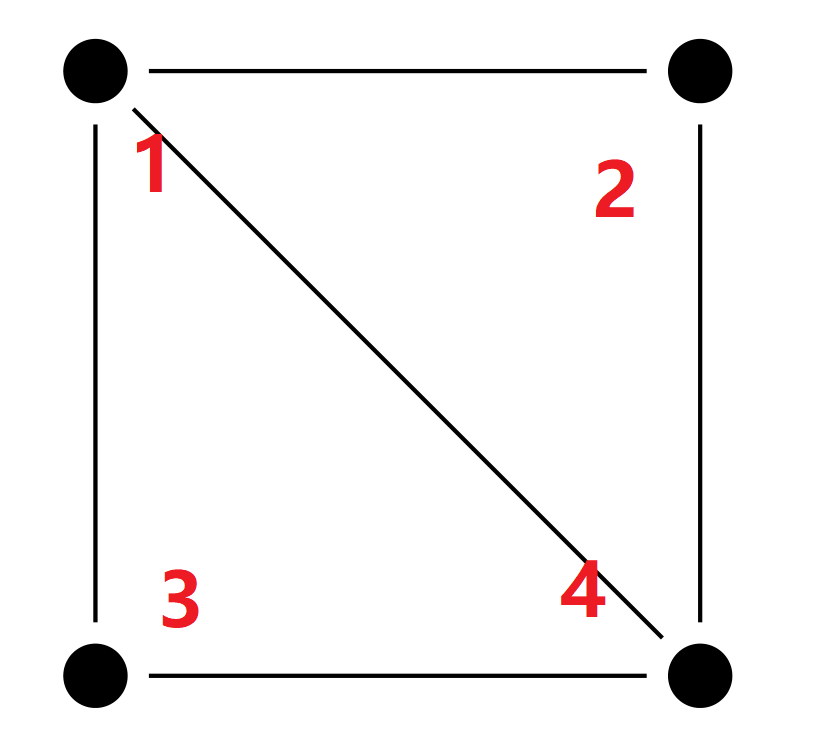
\includegraphics[scale=0.5]{location}
        \end{center}
    let calculate the number of all colouring combination which can lead to a 3 colouring graph:\\
    first, let's color node 1, 2 and 4, since these 3 nodes all connect together, they must be colored differently.\\
    There are $ 3! = 6 $ different colouring combination of nodes 1, 2 and 4.\\
    Then, let consider node 3, its color must be different from node 1 and 2, so its color is the same as node 4.\\
    There are only 1 choice.
    Therefore, the probability is $ 6/81 = 7.4\% $
    \item
    There are 5 edges, namely (1, 2) (1, 3) (1, 4) (2, 4) (3, 4)\\
    All possible colouring combination = $ 5^6 = 15625 $\\
    First, let's color (1, 2):\\
    We can choose from any "colour pairs“ (eg, (reg, green)),there are 6 choices.\\
    Second, Let's color (1, 3):\\
    If (1, 2) is colored by (red, green), then (1, 3) must be colored with (red, xx), because others will not be valid\\
    Moreover, consider the conclusion we made in previous question\\
    in order to get a 3-coloring graph, 2, and 3 must be in same color, which is (xx, green) for example.\\
    Therefore, the "colour pairs" for (1, 3) is the same as (1, 2), there are 1 choice.\\
    Third, let's color (1, 4):\\
    color for 1 is fixed, and color for 4 must be different from 2(which is the same color as 3)\\
    Therefore, there are 1 choices\\
    In conclusion, the probability is $ 6/15625 = 0.0384\% $
\end{enumerate}
\end{document}